\documentclass[11pt,a4paper]{article}

% --- Packages ---------------------------------------------------------
\usepackage[margin=1in]{geometry}
\usepackage{times}
\usepackage[utf8]{inputenc}
\usepackage[T1]{fontenc}
\usepackage{amsmath}
\usepackage{graphicx}
\usepackage{booktabs}
\usepackage{caption}
\usepackage{xcolor}
\usepackage{enumitem}
\usepackage[colorlinks=true,linkcolor=blue!50!black,citecolor=blue!50!black,urlcolor=blue!50!black]{hyperref}
\usepackage{titlesec}
\usepackage{fancyhdr}
\usepackage{tikz}
\usepackage{float}
\usetikzlibrary{arrows.meta,positioning}

\titleformat{\section}{\normalfont\large\bfseries}{\thesection}{1em}{}
\titleformat{\subsection}{\normalfont\normalsize\bfseries}{\thesubsection}{1em}{}

% --- Shared TikZ styles for the architecture diagram (Section~\ref{sec:architecture}). ---
\tikzset{
  stage/.style={rectangle, rounded corners=2pt, draw=black!55, thick,
    fill=black!4, minimum height=0.9cm, text width=2.6cm, align=center,
    font=\scriptsize, inner sep=2pt},
  accentstage/.style={stage, draw=blue!60, fill=blue!8, line width=1pt},
  pipearrow/.style={-{Stealth[length=2mm,width=1.6mm]}, thick, black!65},
}
\newcommand{\archfig}[3]{%
  \begin{figure}[H]
  \centering
  \resizebox{\linewidth}{!}{#2}
  \caption{#1}
  \label{#3}
  \end{figure}%
}

\pagestyle{fancy}
\fancyhf{}
\fancyhead[L]{\small SENTINEL --- Project Progress Report}
\fancyhead[R]{\small \thepage}
\renewcommand{\headrulewidth}{0.3pt}

\setlength{\parskip}{0.4em}
\setlength{\parindent}{0pt}

% --- Title (kept short; full cover-page details are set directly in the
% titlepage environment below, not via \author/\date, since this is a lab
% report -- cover page and content are separate, unlike a research paper
% that folds title/authors/affiliation straight into the first page.) ----

\title{\textbf{SENTINEL}}

\begin{document}

% --- Cover page ---------------------------------------------------------
\begin{titlepage}
\thispagestyle{empty}
\centering
\vspace*{1.5cm}

{\LARGE \textbf{Khulna University of Engineering \& Technology}}\\[0.3em]
{\large Department of Computer Science and Engineering}

\vspace{1.5cm}

{\large \textsc{Project Progress Report}}

\vspace{2cm}

{\Huge \textbf{Sentinel}}

\vspace{0.8cm}

{\large A Real-Time 3D Graphics Renderer of a\\Night-Time Military Base, Built Entirely by Code}

\vspace{3cm}

{\large \textbf{Md. Shifat Hasan (2107067)}}

\vfill

\begin{tabular}{rl}
\textbf{Course:} & Computer Graphics and Image Processing Laboratory (CSE 4102) \\[0.3em]
\textbf{Year / Term:} & 4th Year, 1st Term \\[0.3em]
\textbf{Lab Group:} & B1 \\[0.3em]
\textbf{Instructors:} & Md. Tajmilur Rahman \\
& Md. Mubtashim Abrar Nihal \\
\end{tabular}

\vspace{2cm}

{\large September 23, 2026}

\end{titlepage}

\tableofcontents
\newpage

% --- Abstract -------------------------------------------------------------
\begin{abstract}
\noindent
\textbf{SENTINEL} is a real-time, hand-built renderer of a small
night-time Forward Operating Base (FOB), written from scratch in the
Odin programming language on top of the OpenGL core profile, hand-written
GLSL, and GLFW, with no game engine, no scene-graph library, and no
imported models, textures, or precomputed geometry of any kind. This
report documents progress as of the current milestone: a custom,
theme-agnostic OpenGL abstraction layer; a procedural geometry system
restricted to three base primitives (cube, tetrahedron, plane), from
which every other shape in the scene -- cylinders, cones, wedges, and
full composite objects -- is assembled at runtime by combining primitive
instances through matrix transforms; a hand-rolled parent/local-transform
scene hierarchy supporting nested articulation; nine procedurally
generated scene objects, several with multi-level hierarchical children;
a free-fly camera with live-switchable perspective and orthographic
projections; an automatic \emph{Patrol Mode} that animates the scene
through pure time-driven formulas; and an interactive \emph{Inspection
Mode} that supports object selection (by keyboard cycling and real
mouse-ray picking), and live translate/rotate editing of any selected
object's transform. All geometry, object placement, and animation is
generated by runtime formulas -- nothing is hardcoded as a literal table
of numbers, and nothing is cached as though it were static data. The
project is organized into independently testable Odin packages, with 49
automated unit tests currently passing and a headless screenshot-capture
mechanism used throughout development for self-verification. Illumination,
shading, culling/hidden-surface-removal demonstrations, and the ray/path/
photon-tracing components of the course syllabus are planned for the next
development phase and are intentionally out of scope for this report.
\end{abstract}

\vspace{1em}

% =======================================================================
\section{Introduction}
% =======================================================================

Modern real-time computer graphics rests on a small set of recurring
ideas -- procedural construction of geometry, hierarchical transformation
of that geometry, camera and projection mathematics, and, ultimately,
illumination -- that are far better understood by building a renderer
from first principles than by treating a graphics engine as a black box.
\textbf{SENTINEL} is a course project built on exactly that premise: a
small, self-contained, night-time military base scene, rendered by a
renderer whose every mesh, object placement, and animation is produced by
code executed at runtime, never authored as a static asset or a literal
data table.

The \emph{Forward Operating Base} theme was chosen deliberately. A small
military outpost is a natural setting for a handful of clearly countable,
standard-complexity structures (a watchtower, a perimeter fence, a jeep,
a bunker, a radar installation, barracks, a crate stack, a tank, and a
gun emplacement) that will, in a later phase of the project, be watched
over by considerably more independent light sources than there are
objects -- floodlights, fence lamps, headlights, and window glow -- which
is exactly the object-to-light ratio the course's illumination
requirements call for. Independently of illumination, the same nine
objects already give this report's milestone a rich, varied
demonstration of procedural geometry and, in three cases, multi-level
transform hierarchies.

\subsection{Objectives}
This stage of the project set out to:
\begin{enumerate}[nosep]
  \item Build a minimal, theme-agnostic OpenGL abstraction layer (shader
        compilation and uniform upload, vertex/index buffers, a vertex
        array description, and GL error checking) in Odin, with no
        third-party graphics or math library beyond Odin's own standard
        \texttt{core:math/linalg} package.
  \item Implement procedural mesh generation restricted to exactly three
        base primitives -- cube, tetrahedron, and plane -- each with
        vertex positions computed from a runtime size parameter, never a
        literal coordinate list, plus a general instancing/combination
        mechanism capable of assembling every other required shape from
        these three.
  \item Construct a minimum of six (targeted: nine) standard-complexity
        scene objects entirely from this procedural system, including at
        least one deep parent/child hierarchy suitable for demonstrating
        correct nested-transform composition.
  \item Implement a free-fly camera with both perspective and
        orthographic projections, switchable at runtime.
  \item Implement two operating modes required by the course -- an
        automatic ``loop'' mode and an interactive, user-controlled mode
        -- sharing a single rendering code path, differing only in what
        drives the transform matrices each frame.
  \item Verify every claim above with automated tests and reproducible,
        headless screenshot evidence, rather than relying on visual
        inspection alone.
\end{enumerate}

\subsection{Scope of this report}
This is an interim \emph{progress} report, not a final project report.
It documents the state of the renderer as of the current milestone --
procedural geometry, the transform hierarchy, the camera system, and
both operating modes -- and is deliberately scoped to that milestone.
Illumination models, multi-light support, shading-method comparison,
back-face culling and hidden-surface-removal demonstrations, and the
ray-tracing/path-tracing/photon-mapping components of the syllabus are
addressed in Section~\ref{sec:future-work} as planned work for the next
development phase, and are not claimed as complete here.

% =======================================================================
\section{Technology Stack and Development Environment}
% =======================================================================

\begin{table}[H]
\centering
\caption{Technology stack.}
\label{tab:stack}
\begin{tabular}{ll}
\toprule
\textbf{Component} & \textbf{Choice} \\
\midrule
Language & Odin \\
Graphics API & OpenGL, core profile (version 3.3) \\
Shading language & Hand-written GLSL (no third-party shader code) \\
Windowing / input & GLFW, via Odin's \texttt{vendor:glfw} bindings \\
GL function loading & Odin's \texttt{vendor:OpenGL} loader \\
Vector / matrix math & Odin's own \texttt{core:math/linalg} \\
Build system & The Odin compiler's own package-based build (\texttt{odin build} / \texttt{odin test}) \\
\bottomrule
\end{tabular}
\end{table}

No game engine, scene-graph library, or third-party math library is
used anywhere in the project. \texttt{core:math/linalg} supplies vector
and matrix \emph{types} and standard operations (translation, rotation,
projection matrices, and so on) -- everything object-specific,
including the entire scene hierarchy, is hand-written. No textures or
imported 3D models are used at any point; every colour in the current
build is a flat, per-object material value.

% =======================================================================
\section{Design Constraints and Principles}
\label{sec:constraints}
% =======================================================================

The project is governed by a small number of hard constraints, stated
here because they directly shape the architecture described in the
remaining sections:

\begin{itemize}[nosep]
  \item \textbf{No precomputed data.} Vertex positions, object
        placements, camera paths, and animation values are never stored
        as literal arrays of numbers. Everything is produced by a
        runtime formula -- a loop, a trigonometric function, a spacing
        rule -- evaluated as needed. Small \emph{parameters} that feed
        such a formula (a radius, a count, a height, a colour) are
        permitted; literal position or vertex \emph{tables} are not.
  \item \textbf{Only three base primitives.} The only mesh shapes
        generated directly are a cube (general box), a tetrahedron, and
        a plane, each with procedurally computed vertices. Every other
        shape -- a cylinder-like leg, a cone-like roof, a wedge, a
        composite object -- is assembled at runtime by combining
        multiple instances of these three via matrix transforms, never
        by a dedicated shape-specific vertex generator.
  \item \textbf{No scene-graph library.} The transform hierarchy
        described in Section~\ref{sec:hierarchy} is a small, hand-rolled
        parent/local-transform system, not an imported dependency.
  \item \textbf{No imported assets.} All geometry is procedural; no 3D
        model files or textures are loaded.
  \item \textbf{A single render path for both operating modes.} The two
        modes described in Section~\ref{sec:modes} differ only in what
        \emph{drives} the transform matrices each frame (a scripted
        formula versus live user input) -- never in how a frame is
        actually drawn.
\end{itemize}

% =======================================================================
\section{System Architecture}
\label{sec:architecture}
% =======================================================================

The codebase is organized into independent Odin packages with clear
responsibilities, rather than one flat collection of source files.
Figure~\ref{fig:architecture} shows the dependency structure.

\begin{itemize}[nosep]
  \item \textbf{\texttt{Engine}} -- a theme-agnostic OpenGL wrapper
        (shader compilation and typed uniform upload, vertex/index
        buffers, a vertex array/layout description, a minimal renderer,
        and GL error checking). Knows nothing about the FOB theme.
  \item \textbf{\texttt{Geometry}} -- theme-agnostic procedural mesh
        generation, restricted to the three base primitives from
        Section~\ref{sec:constraints}, plus the mesh-combination
        primitive every composite shape is built from.
  \item \textbf{\texttt{Camera}} -- a free-fly camera, both projection
        matrices, and the (theme-agnostic) automatic patrol-path
        mathematics, with no GLFW or windowing dependency.
  \item \textbf{\texttt{Scene}} -- the SENTINEL-specific transform
        hierarchy and the procedural construction of all nine scene
        objects, built on top of \texttt{Geometry}.
  \item \textbf{\texttt{Source} (application)} -- the entry point: window
        and GL context creation, the main render loop, input handling,
        and the logic that switches between the two operating modes.
\end{itemize}

\begin{figure}[H]
\centering
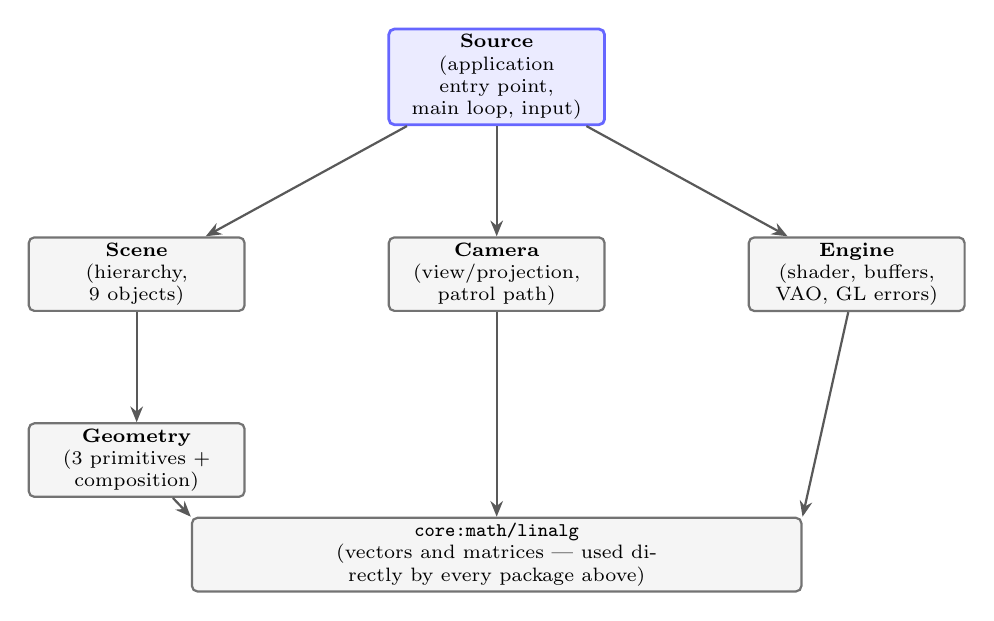
\begin{tikzpicture}[node distance=14mm and 18mm]
\node[accentstage] (source) {\textbf{Source}\\(application entry point,\\main loop, input)};
\node[stage, below left=of source] (scene) {\textbf{Scene}\\(hierarchy,\\9 objects)};
\node[stage, below=of source] (camera) {\textbf{Camera}\\(view/projection,\\patrol path)};
\node[stage, below right=of source] (engine) {\textbf{Engine}\\(shader, buffers,\\VAO, GL errors)};
\node[stage, below=of scene] (geometry) {\textbf{Geometry}\\(3 primitives +\\composition)};
\node[stage, below=26mm of camera, text width=7.6cm] (linalg) {\texttt{core:math/linalg}\\(vectors and matrices --- used directly by every package above)};

\draw[pipearrow] (source) -- (scene);
\draw[pipearrow] (source) -- (camera);
\draw[pipearrow] (source) -- (engine);
\draw[pipearrow] (scene) -- (geometry);
\draw[pipearrow] (geometry) -- (linalg.north west);
\draw[pipearrow] (camera) -- (linalg.north);
\draw[pipearrow] (engine) -- (linalg.north east);
\end{tikzpicture}
\caption{Package dependency structure. \texttt{Engine} and
\texttt{Geometry} are theme-agnostic and know nothing about SENTINEL's
own objects; \texttt{Scene} and \texttt{Camera} sit above them, and the
\texttt{Source} application ties everything together. Two minor edges
are omitted for readability: \texttt{Geometry} also depends on
\texttt{Engine} for its GPU buffer types, and \texttt{Scene} depends on
\texttt{core:math/linalg} directly in addition to via \texttt{Geometry}.}
\label{fig:architecture}
\end{figure}

The \texttt{Engine} layer began from a smaller, earlier learning-project
skeleton and was audited and confirmed compatible with this project's
constraints rather than rewritten outright: its uniform-upload procedures
already operate directly on \texttt{core:math/linalg} matrix types.

% =======================================================================
\section{Procedural Geometry Generation}
\label{sec:geometry}
% =======================================================================

\subsection{Base primitives}
Three primitives are generated directly, each parametrized entirely by a
runtime size argument:

\begin{itemize}[nosep]
  \item \textbf{Cube} -- full width/height/depth given as parameters;
        loops over its six faces, computing each face's four corners
        from a fixed sign-combination pattern scaled by the given
        half-extents. 24 vertices (four per face, for flat per-face
        normals), 12 triangles.
  \item \textbf{Tetrahedron} -- four corners at alternating corners of a
        cube of the given size (the standard regular-tetrahedron-inside-
        a-cube parametrization), scaled by a runtime size argument. 12
        vertices, 4 triangles.
  \item \textbf{Plane} -- a single quad of the given width/height in the
        local $XY$ plane, facing $+Z$. 4 vertices, 2 triangles.
\end{itemize}

Every generator computes a geometric normal from the winding of the
vertices it produces and automatically orients that winding so the
stored normal points outward from the primitive's own centre -- so no
face's winding is ever hand-derived and hardcoded.

\subsection{Composition via runtime transforms}
A single mesh-combination primitive copies one mesh's vertices and
indices into another, applying a transform matrix to each copied
position (and the corresponding inverse-transpose normal matrix to each
copied normal, so normals remain correct under non-uniform scale). Every
shape beyond the three base primitives -- a cylinder-like tower leg, a
radar dish, a wheel rim, a sandbag ring, a cone-like roof -- is built by
calling this combination primitive repeatedly at runtime, most commonly
in one of two patterns:

\begin{itemize}[nosep]
  \item \textbf{Ring composition.} $N$ copies of a small box (or plane)
        segment are placed around a circle by a runtime loop that
        computes a rotation matrix per segment -- a low-poly
        approximation of a cylinder, cone, or ring, with the segment
        count itself a small, freely chosen parameter (this project uses
        6--10 segments per ring, consistent with its low-poly visual
        style).
  \item \textbf{Angled panel composition.} A single box, scaled thin and
        rotated by an angle solved from two geometric reference points
        (for example, a roof's rise and run), used for sloped surfaces
        such as roof slabs and glacis plates.
\end{itemize}

No shape in the scene has its vertex data written out as a literal
coordinate list, and no composite mesh is built once and cached; each
object's geometry is (re)constructed by these same runtime formulas
every time the program starts.

% =======================================================================
\section{Scene Composition}
\label{sec:scene}
% =======================================================================

Nine objects are currently built, exceeding the minimum requirement of
six. Table~\ref{tab:objects} lists each object, its child nodes (if
any), and the composition technique used to build it.

\begin{table}[H]
\centering
\caption{The nine SENTINEL scene objects.}
\label{tab:objects}
\small
\begin{tabular}{p{2.6cm}p{4.4cm}p{6.4cm}}
\toprule
\textbf{Object} & \textbf{Child nodes} & \textbf{Notes} \\
\midrule
Watchtower & Floodlight head & Four legs, platform, railing ring, and a
four-slab pyramid roof; the head is a separate child node so it can
rotate independently. \\
Perimeter fence \& gate & Gate & A full rectangular loop of posts and
panels generated by walking the fence boundary with a parametric
formula, leaving a gap for the gate. \\
Armored jeep & Windshield, left/right headlight & Body, cabin, hood, and
four ring-composed wheels. \\
Sandbag bunker & --- & A U-shaped wall of two stacked, staggered rows of
ring-composed ``sandbags.'' \\
Radar mast & Dish, beacon & A tilted, ring-composed dish and a beacon,
each a separate child for independent animation. \\
Barracks hut & Three windows & Box body with a two-slab wedge roof; the
windows are child nodes on the rear wall. \\
Cargo crate stack & --- & Six crates, each with a size/rotation/offset
determined by a deterministic function of its position in the stack. \\
Battle tank & Turret $\rightarrow$ Barrel, Periscope & \textbf{The
project's deepest hierarchy}: hull (root) $\rightarrow$ turret (child)
$\rightarrow$ barrel and periscope (grandchildren of the hull). \\
Gun emplacement & --- & A sandbag ring, a three-leg tripod, and a gun
body; deliberately static, with no children. \\
\bottomrule
\end{tabular}
\end{table}

Figures~\ref{fig:patrol-overview} and~\ref{fig:inspection-overview} show
the current renderer output. Every object is shown with a single flat
colour and no lighting model applied -- illumination is explicitly out
of scope for this milestone (Section~\ref{sec:future-work}), so what is
visible here is exactly the procedural geometry and the transform
hierarchy this report documents, with nothing added on top.

\begin{figure}[H]
\centering
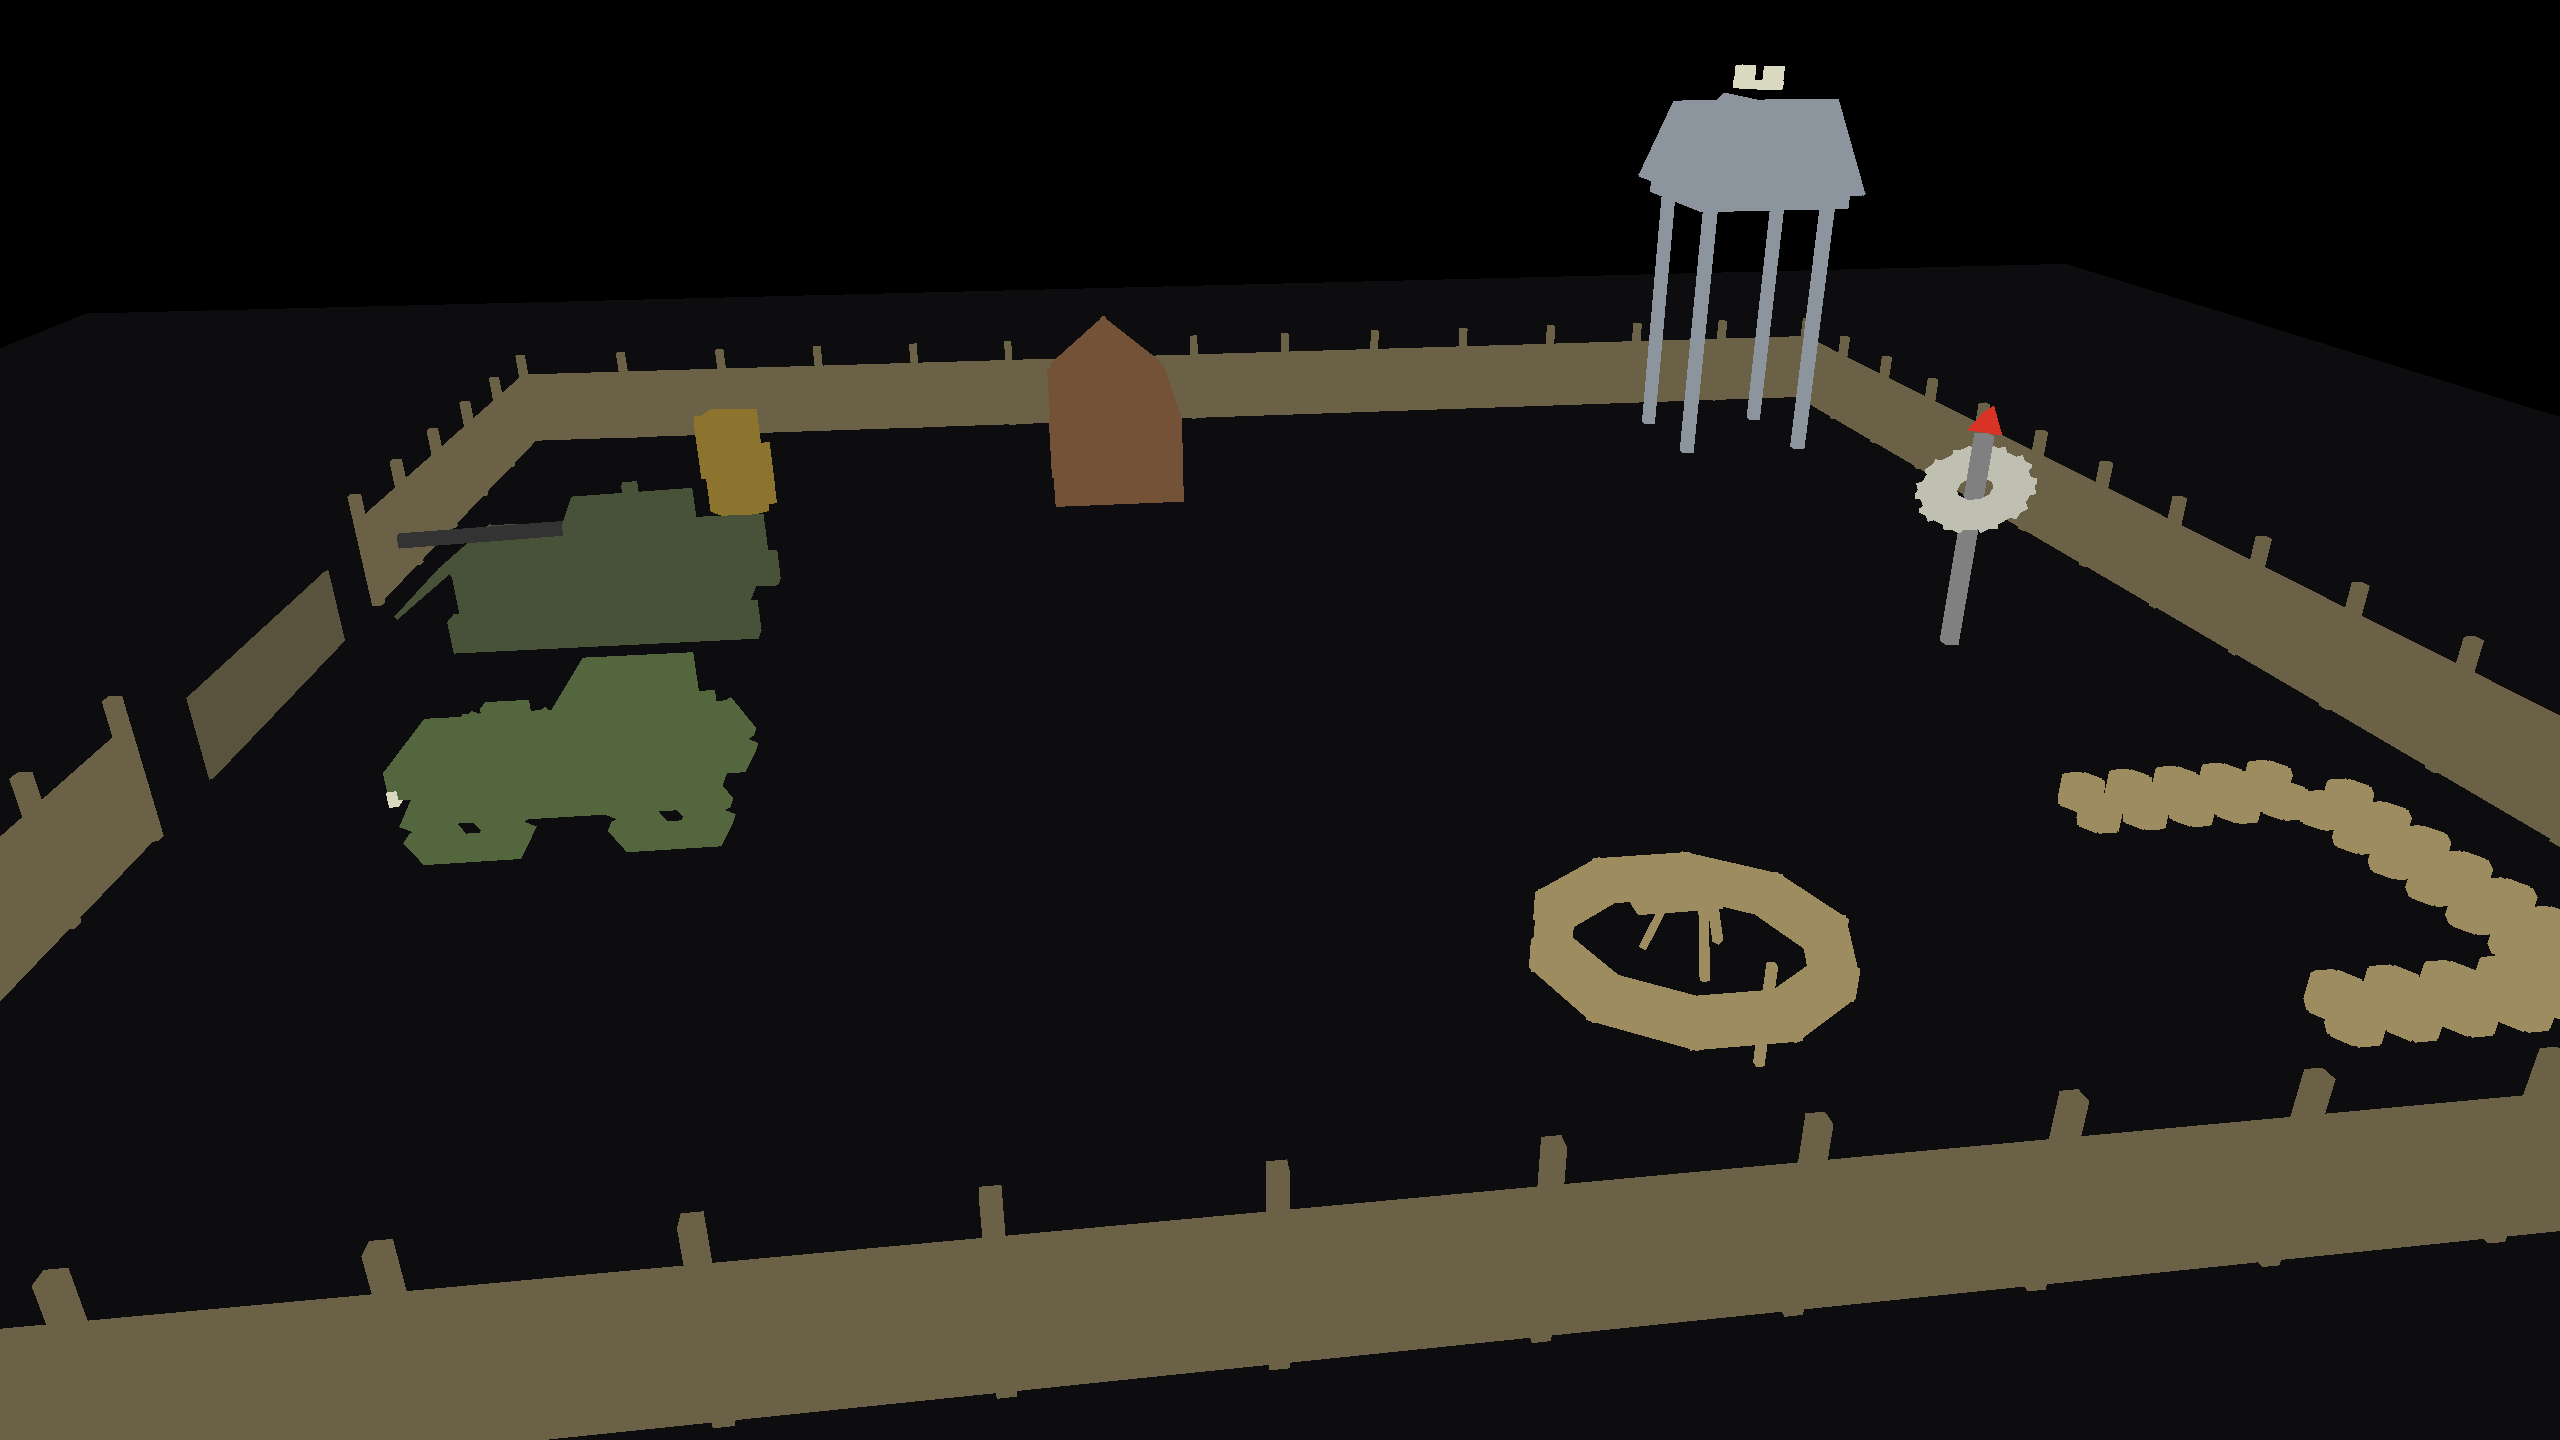
\includegraphics[width=0.92\textwidth]{assets/patrol_overview.png}
\caption{Patrol Mode: the automatic, formula-driven camera circling the
base. Every object is procedurally generated; colours are flat per-object
materials with no illumination applied at this stage.}
\label{fig:patrol-overview}
\end{figure}

\begin{figure}[H]
\centering
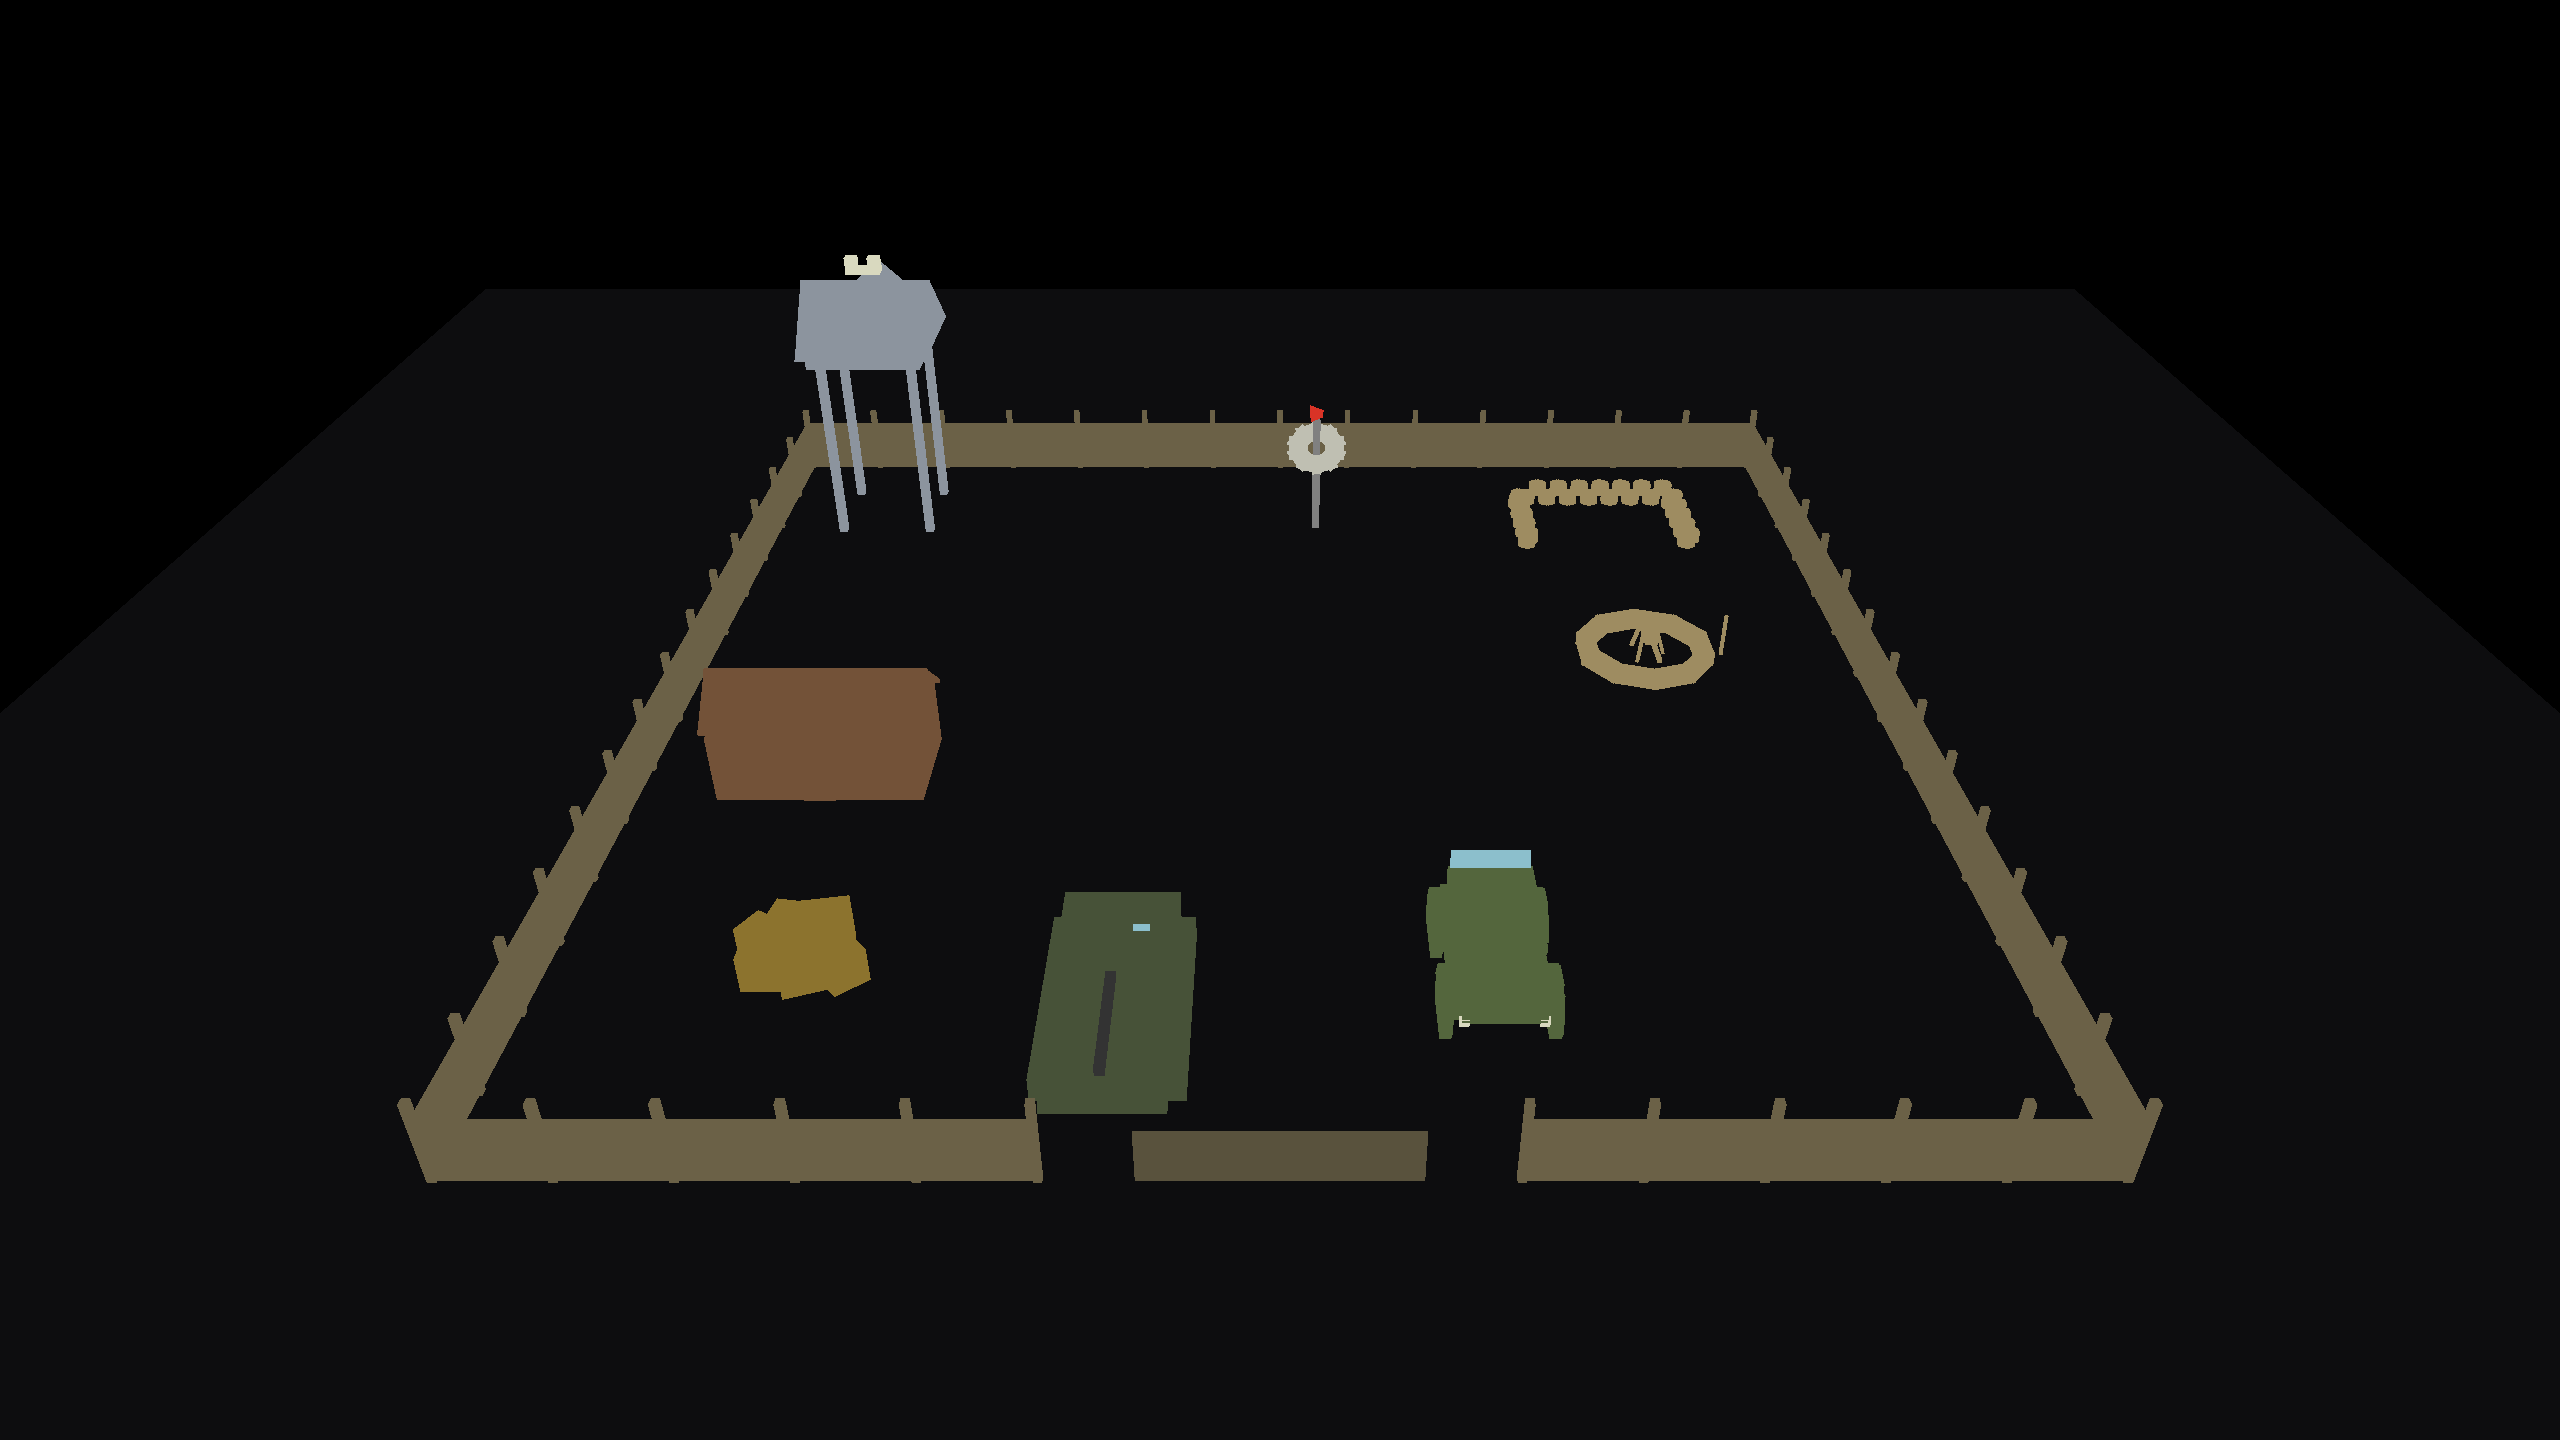
\includegraphics[width=0.92\textwidth]{assets/inspection_overview.png}
\caption{Inspection Mode's default free-fly view of the same scene.}
\label{fig:inspection-overview}
\end{figure}

% =======================================================================
\section{Transform Hierarchy System}
\label{sec:hierarchy}
% =======================================================================

Rather than an imported scene-graph library, SENTINEL uses a small,
flat array of nodes, each storing a name, an optional parent index, a
local transform (position, Euler rotation, scale), and its own mesh and
material. Using a flat array with integer parent indices -- rather than
a tree of pointers -- means a node's index remains valid across the
underlying array's own growth as more nodes are added.

Every node's world matrix is computed by a single top-down pass over the
array: a root node's world matrix is simply its own local matrix; any
other node's world matrix is its parent's (already-computed) world
matrix multiplied by its own local matrix. Nodes are guaranteed to be
added to the array only after their parent already exists, so this
single pass is always sufficient -- no second pass or explicit
topological sort is required. This computation is performed fresh every
frame, never cached, so that any change to a node's local transform
(whether from an automatic animation or an interactive edit) is
correctly reflected the very next frame it is drawn, and correctly
propagates to every descendant.

This mechanism is exercised most thoroughly by the battle tank's
hull~$\rightarrow$~turret~$\rightarrow$~\{barrel, periscope\} chain
(Table~\ref{tab:objects}): rotating the hull carries the turret (and
everything mounted on it) with it, while subsequently rotating the
turret independently moves only the turret and its own children,
without disturbing the hull. Correct composition through this kind of
nested chain is verified directly by automated tests
(Section~\ref{sec:testing}).

% =======================================================================
\section{Camera System and Projections}
\label{sec:camera}
% =======================================================================

A single camera type supports both a free-fly mode (position, yaw, and
pitch, driven by keyboard and mouse input) and a formula-driven
automatic path, and can build either a perspective or an orthographic
projection matrix from the same state. Both projection matrices are
constructed directly from Odin's \texttt{core:math/linalg} package, and
both are switchable live, at runtime, without interrupting rendering.
When switching from perspective to orthographic, the orthographic
view volume's size is derived from the camera's current distance to a
fixed scene-focus point, so the visible framing does not jump at the
moment of the switch.

The automatic patrol path is itself a pure formula: the camera's
position moves along a circle of fixed radius around the base (with a
small sinusoidal height bob), while its look direction is solved, every
frame, to aim at a slowly drifting target point near the base's centre
-- so, consistent with Section~\ref{sec:constraints}, no camera
waypoint is ever stored as data; the entire path is recomputed from the
current animation time on every frame.

% =======================================================================
\section{Operating Modes}
\label{sec:modes}
% =======================================================================

The course requires two runtime-toggleable operating modes: an automatic
loop mode and an interactive, user-controlled mode. Both are implemented
and share the exact same drawing code path (Section~\ref{sec:constraints});
they differ only in what supplies the values written into each frame's
transform matrices.

\subsection{Patrol Mode (automatic)}
With zero user input, the camera follows the automatic path described in
Section~\ref{sec:camera} while several scene nodes are animated by their
own independent, pure time-driven formulas: the watchtower's floodlight
head sweeps back and forth, the radar dish spins continuously, the tank
turret slowly scans, and the jeep's headlight nodes dip periodically.
Every one of these is a rotation of an existing node's local transform,
computed fresh each frame from a shared animation clock -- never a
stored keyframe sequence.

\subsection{Inspection Mode (interactive)}
Inspection Mode provides a free-fly camera (keyboard movement and mouse
look) plus object manipulation:

\begin{itemize}[nosep]
  \item \textbf{Selection.} Twelve nodes are selectable -- the nine root
        objects plus three notable child nodes (the tank turret, the
        watchtower's floodlight head, and the radar dish) chosen
        specifically to demonstrate independent child-transform editing.
        Selection can step through this list via the keyboard, or a node
        can be picked directly: a ray is unprojected from the centre of
        the screen through the inverse of the current view-projection
        matrix, and tested against each selectable node's own
        axis-aligned bounding box (computed once from that node's local
        geometry, then transformed into the node's current world space),
        with the nearest intersection winning.
  \item \textbf{Translate and rotate.} The selected node's \emph{local}
        transform can be edited live; because children are always
        recomposed from their parent's current world matrix
        (Section~\ref{sec:hierarchy}), editing a parent's local
        transform is sufficient for every descendant to follow
        automatically, with no additional propagation step.
  \item \textbf{Reset.} The selected object, or every object at once,
        can be restored to the transform it had when the program
        started.
  \item \textbf{Projection toggle.} Perspective and orthographic
        projection can be switched live in either mode.
\end{itemize}

Switching between modes does not desynchronize state: leaving Inspection
Mode for Patrol Mode resumes the automatic camera path from the nearest
point on its circular route to wherever the free camera currently is,
rather than jumping to an unrelated point on the path.

% =======================================================================
\section{Verification and Testing Methodology}
\label{sec:testing}
% =======================================================================

Because this project has no dedicated graphical debugger and the
renderer's own window cannot always be watched interactively during
development, two complementary verification mechanisms are used
throughout:

\begin{itemize}[nosep]
  \item \textbf{Automated unit tests.} Odin's built-in testing framework
        (\texttt{odin test}) is used across every package. As of this
        report, \textbf{49 tests pass}, covering: camera and projection
        mathematics (including empirical checks of coordinate-handedness
        and rotation-direction conventions); procedural-geometry
        correctness (each generator's triangle winding matches its own
        stored normals, normals point outward from the primitive's
        centre, and vertex/index counts are exact); the transform
        hierarchy (including a dedicated multi-level test confirming
        that rotating an intermediate node correctly carries its
        children through the resulting composed transform); and the
        mouse-picking mathematics used by Inspection Mode (ray/box
        intersection, screen-to-world ray construction, and nearest-hit
        selection).
  \item \textbf{Headless, reproducible screenshot capture.} The
        application supports a command-line flag that renders a fixed
        number of frames, saves the resulting framebuffer to an image
        file, and exits -- allowing the renderer's actual output to be
        inspected and compared frame-for-frame without a live,
        interactively-watched session. This mechanism produced
        Figures~\ref{fig:patrol-overview} and~\ref{fig:inspection-overview}.
\end{itemize}

% =======================================================================
\section{Current Progress Status}
\label{sec:status}
% =======================================================================

Table~\ref{tab:status} summarizes progress against the full course
syllabus. Topics in the upper block are complete and demonstrated by
this report; topics in the lower block are planned for the next phase of
development (Section~\ref{sec:future-work}).

\begin{table}[H]
\centering
\caption{Progress against the course syllabus.}
\label{tab:status}
\begin{tabular}{p{6.2cm}p{5.2cm}c}
\toprule
\textbf{Syllabus topic} & \textbf{Where it lives} & \textbf{Status} \\
\midrule
Display/input devices, graphics pipeline & GLFW window and input; a
custom OpenGL pipeline & Complete \\
Scan conversion, polygon filling & GPU rasterization of correctly wound,
procedurally generated triangle meshes & Complete \\
3D primitives, basic \& composite transformations & Procedural
primitive generators; hierarchical transform chains
(Sections~\ref{sec:geometry}--\ref{sec:hierarchy}) & Complete \\
Classical / computer viewing, projective transformation & Free-fly
camera; perspective and orthographic projections, toggled live
(Section~\ref{sec:camera}) & Complete \\
\midrule
Local / global illumination, polygon shading methods & --- & Planned \\
Light types (point, spot, area, directional) & --- & Planned \\
Back-face culling & --- & Planned \\
Hidden surface removal & --- & Planned \\
Ray tracing & --- & Planned \\
Path tracing & --- & Planned \\
Photon mapping\textsuperscript{$\dagger$} & --- & Planned \\
\bottomrule
\end{tabular}

\vspace{0.3em}
\raggedright
\footnotesize\textsuperscript{$\dagger$}Planned as a written explanation
of how the technique would extend the ray-traced component, not a live
implementation (Section~\ref{sec:future-work}).
\end{table}

Beyond the syllabus mapping, current functional status is: nine
procedurally generated objects (target met, minimum of six exceeded);
one three-level transform hierarchy (tank hull~$\rightarrow$~turret~
$\rightarrow$~barrel/periscope) plus several two-level hierarchies,
all verified by automated tests; both required operating modes
implemented and sharing a single render path; both projection modes
switchable at runtime; and 49 automated tests passing with no known
failures.

% =======================================================================
\section{Remaining Work}
\label{sec:future-work}
% =======================================================================

The following syllabus areas are planned for the next phase of
development, in roughly the order they will be undertaken:

\begin{enumerate}[nosep]
  \item \textbf{Multi-light illumination.} A Blinn-Phong local
        illumination model (ambient, diffuse, specular, and emission
        terms) evaluated over multiple simultaneously active lights,
        with the total active light count planned to exceed the
        nine-object count by a meaningful margin.
  \item \textbf{Light types.} Point, spot, area, and directional lights,
        attached through the existing transform hierarchy so that a
        light parented to a moving or rotating object (for example, the
        tank turret's searchlight, or the jeep's headlights) continues
        to aim and follow correctly.
  \item \textbf{Shading-method comparison.} Flat, Gouraud, and Phong
        shading, switchable live for direct visual comparison.
  \item \textbf{Back-face culling and hidden-surface removal.} A manual,
        normal-based culling test compared directly against hardware
        culling, and the GPU depth buffer's role in hidden-surface
        removal, both made toggleable so the underlying mechanism can be
        demonstrated rather than only its effect.
  \item \textbf{Ray tracing.} A small, genuinely ray-traced element
        (analytic ray/primitive intersection against a compact proxy
        representation of the scene), rather than a purely decorative
        approximation.
  \item \textbf{Path tracing.} A bounded, multi-sample numerical
        integration technique for at least one area-like light source.
  \item \textbf{Photon mapping.} Addressed as a written explanation of
        how the technique would extend the ray-traced component above --
        photon emission, spatial storage, and a gather pass -- rather
        than implemented directly, since it is fundamentally a batch/
        offline technique in tension with this project's own
        every-frame, nothing-cached design principle
        (Section~\ref{sec:constraints}).
  \item \textbf{Final documentation.} A complete build/run guide,
        control reference, and a final report covering the full,
        completed system.
\end{enumerate}

% =======================================================================
\section{Conclusion}
% =======================================================================

At this stage, SENTINEL has a working, procedurally generated scene of
nine objects assembled entirely from three base primitives, a correct
and independently tested hierarchical transform system capable of
multi-level nested articulation, a camera supporting both standard
projections, and two fully functional operating modes -- one automatic
and formula-driven, one interactive -- sharing a single rendering code
path, exactly as the course requires. No geometry, placement, or
animation data is hardcoded anywhere in the project; everything shown in
Figures~\ref{fig:patrol-overview} and~\ref{fig:inspection-overview} is
produced by runtime code. The remaining syllabus topics --
illumination, shading, culling and hidden-surface-removal
demonstrations, and the ray/path/photon-tracing components -- are
scoped and planned (Section~\ref{sec:future-work}) as the next phase of
this project's development.

\vspace{2em}
\begin{thebibliography}{9}

\bibitem{odin}
Odin Programming Language, Official Documentation.
\url{https://odin-lang.org/docs/}

\bibitem{opengl}
Khronos Group. \textit{OpenGL 3.3 Core Profile Specification}.
\url{https://www.khronos.org/registry/OpenGL/specs/gl/glspec33.core.pdf}

\bibitem{glfw}
GLFW: An OpenGL Library for Creating Windows, Contexts, and Surfaces.
\url{https://www.glfw.org/documentation.html}

\end{thebibliography}

\end{document}
